% Disallowed right-leaning red links and four possible pairs of consecutive red links.
% Editable source for this diagram. From this directory, regenerate with:
% latex -interaction=nonstopmode -halt-on-error llrbt-2.tex
% dvisvgm --no-fonts --exact --bbox=papersize --output=llrbt-2.svg llrbt-2.dvi
\documentclass[tikz,border=12pt]{standalone}
\usepackage{lmodern}
\usepackage{tikz}
\usetikzlibrary{arrows.meta,backgrounds,shapes.geometric,patterns}
\definecolor{linkred}{HTML}{B5240A}
\definecolor{noteBlue}{HTML}{0067A5}
\definecolor{softgreen}{HTML}{D8EAD0}
\definecolor{softpurple}{HTML}{D9D1E8}
\definecolor{softpink}{HTML}{F5CECF}
\definecolor{softyellow}{HTML}{FFF2C9}
% Translucent vector layers keep the soft shadow in the DVI-to-SVG export.
\tikzset{
  llrbt shadow layer/.style args={#1/#2}{
    preaction={fill=black,draw=none,fill opacity=#2,
      transform canvas={shift={(3pt,-3pt)},
        scale around=#1:(current path bounding box.center)}}
  },
  llrbt shadow/.style={
    llrbt shadow layer=1.40/0.01,
    llrbt shadow layer=1.35/0.015,
    llrbt shadow layer=1.30/0.025,
    llrbt shadow layer=1.25/0.04,
    llrbt shadow layer=1.20/0.06,
    llrbt shadow layer=1.15/0.08,
    llrbt shadow layer=1.10/0.10,
    llrbt shadow layer=1.05/0.12,
    llrbt shadow layer=1.00/0.14,
    llrbt shadow layer=0.95/0.16,
    llrbt shadow layer=0.90/0.18,
    llrbt shadow layer=0.85/0.20
  }
}
\begin{document}
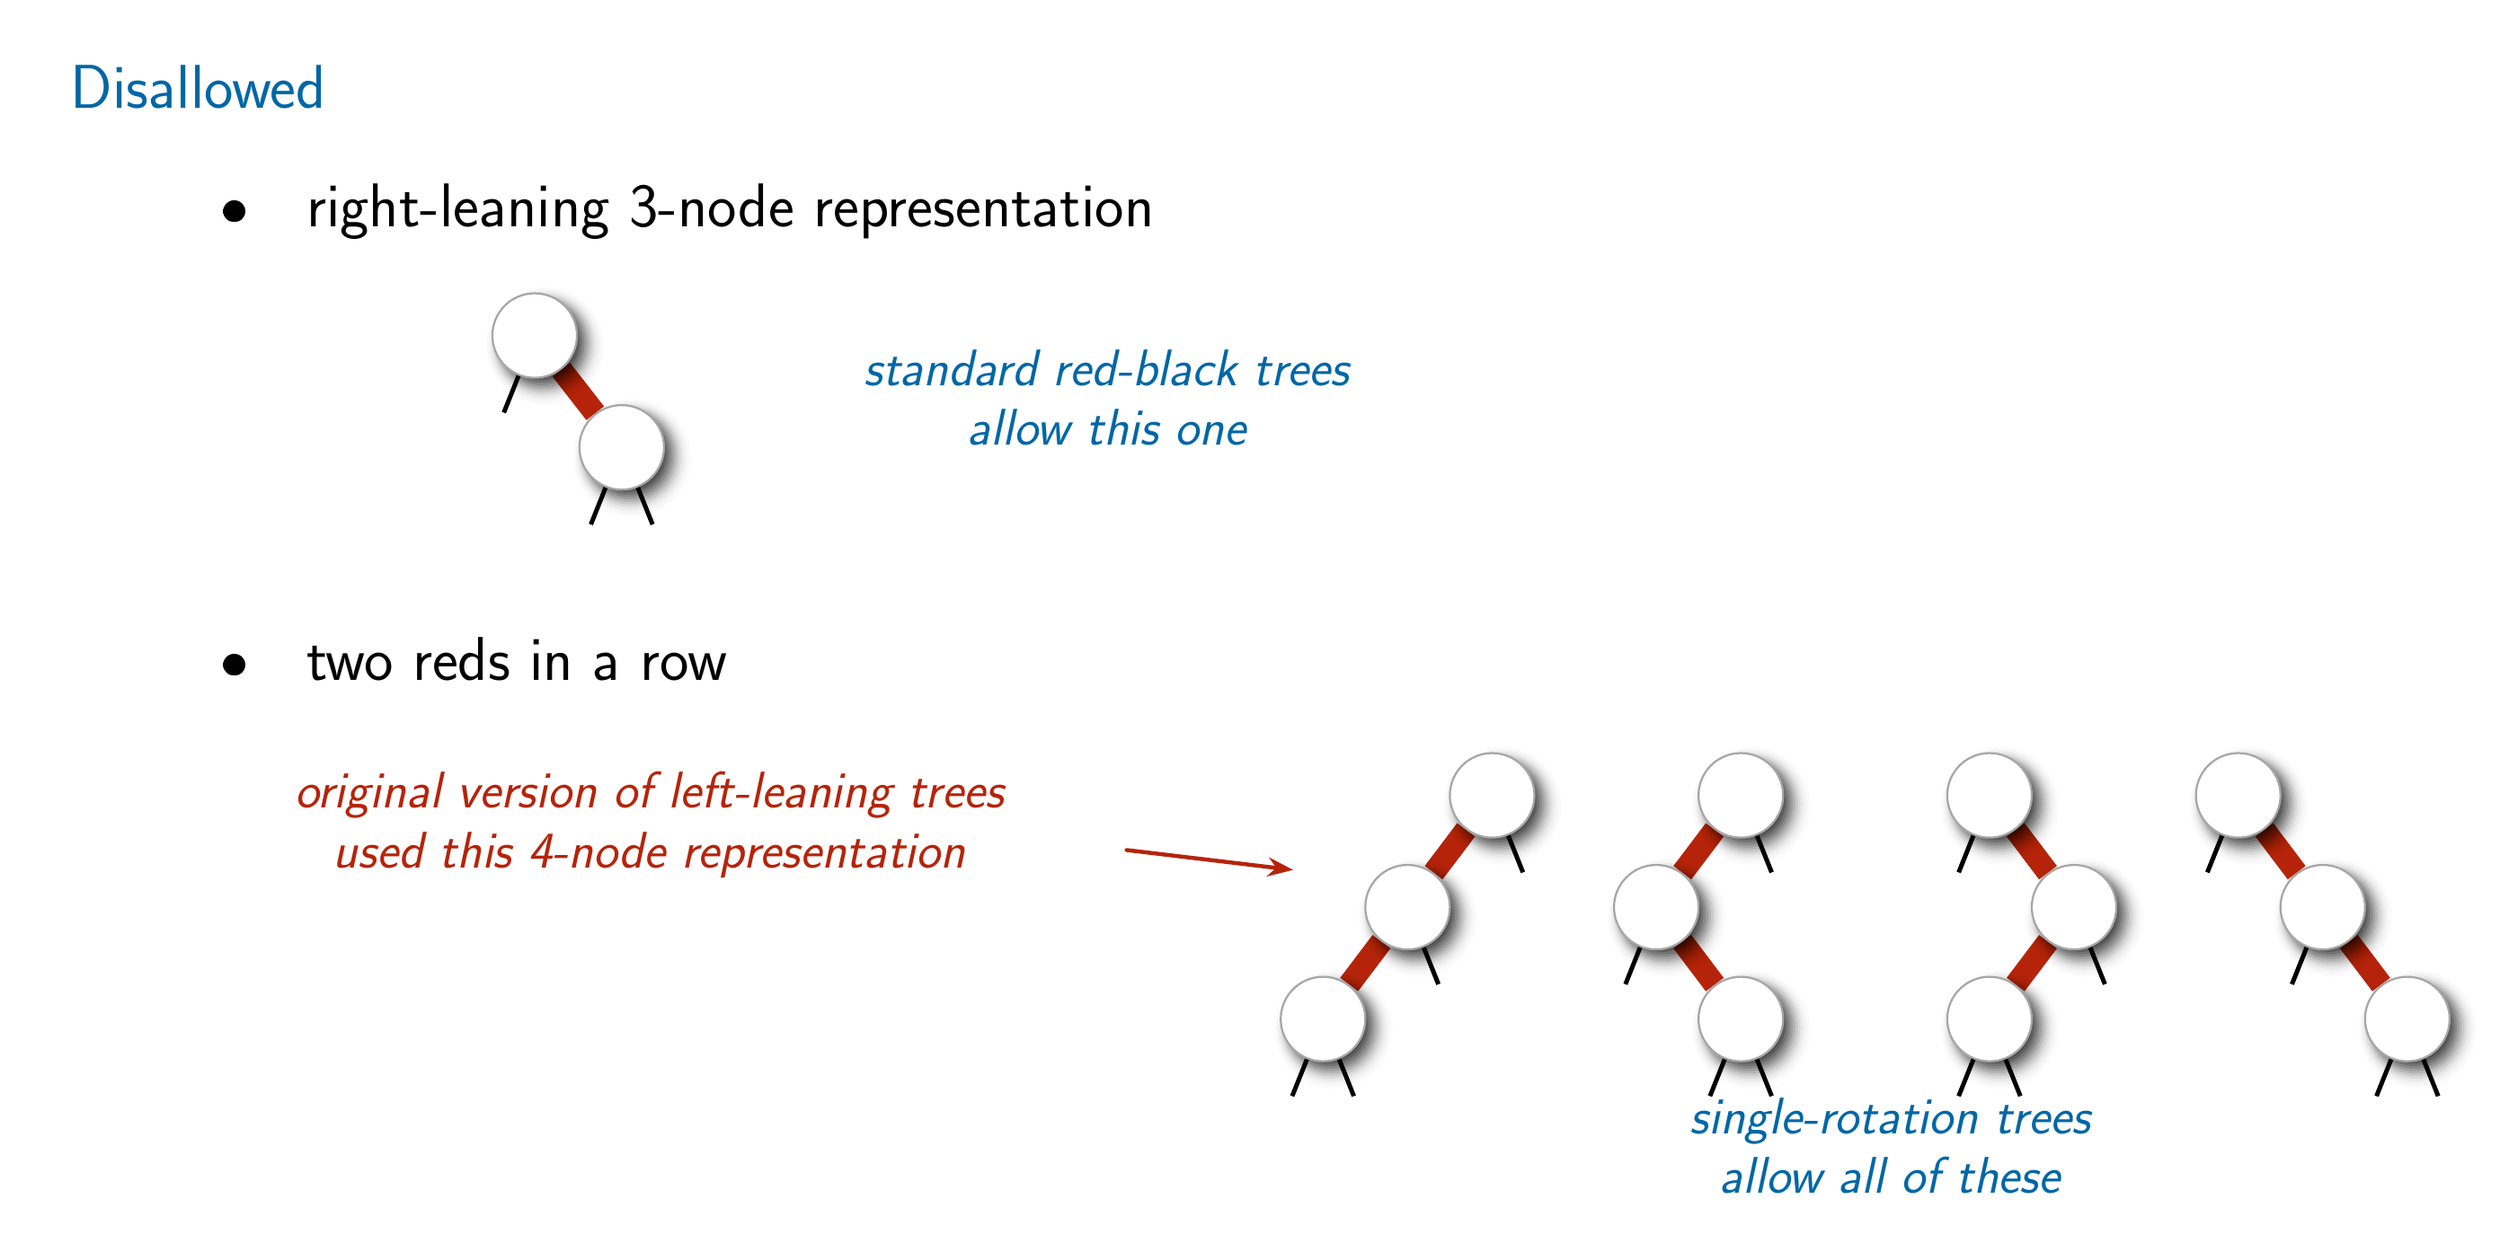
\begin{tikzpicture}[x=1pt,y=-1pt,>=Stealth,line cap=round,line join=round]
\path[use as bounding box] (0,0) rectangle (985,480);
\begin{scope}[on background layer]
\draw[draw=black,line width=1.8pt] (205,125) -- (192.6,156);
\draw[draw=black,line width=1.8pt] (240,170) -- (227.6,201);
\draw[draw=black,line width=1.8pt] (240,170) -- (252.4,201);
\draw[draw=black,line width=1.8pt] (590,310) -- (602.4,341);
\draw[draw=black,line width=1.8pt] (556,355) -- (568.4,386);
\draw[draw=black,line width=1.8pt] (522,400) -- (509.6,431);
\draw[draw=black,line width=1.8pt] (522,400) -- (534.4,431);
\draw[draw=black,line width=1.8pt] (690,310) -- (702.4,341);
\draw[draw=black,line width=1.8pt] (656,355) -- (643.6,386);
\draw[draw=black,line width=1.8pt] (690,400) -- (677.6,431);
\draw[draw=black,line width=1.8pt] (690,400) -- (702.4,431);
\draw[draw=black,line width=1.8pt] (790,310) -- (777.6,341);
\draw[draw=black,line width=1.8pt] (824,355) -- (836.4,386);
\draw[draw=black,line width=1.8pt] (790,400) -- (777.6,431);
\draw[draw=black,line width=1.8pt] (790,400) -- (802.4,431);
\draw[draw=black,line width=1.8pt] (890,310) -- (877.6,341);
\draw[draw=black,line width=1.8pt] (924,355) -- (911.6,386);
\draw[draw=black,line width=1.8pt] (958,400) -- (945.6,431);
\draw[draw=black,line width=1.8pt] (958,400) -- (970.4,431);
\end{scope}
\node[llrbt shadow,circle,draw=black!35,fill=white,text=noteBlue,minimum size=34pt,inner sep=0pt,line width=0.8pt,font=\sffamily\fontsize{18}{21.6}\selectfont,font=\sffamily\itshape\fontsize{18}{22}\selectfont] (ar) at (205,125) {};
\node[llrbt shadow,circle,draw=black!35,fill=white,text=noteBlue,minimum size=34pt,inner sep=0pt,line width=0.8pt,font=\sffamily\fontsize{18}{21.6}\selectfont,font=\sffamily\itshape\fontsize{18}{22}\selectfont] (al) at (240,170) {};
\node[llrbt shadow,circle,draw=black!35,fill=white,text=noteBlue,minimum size=34pt,inner sep=0pt,line width=0.8pt,font=\sffamily\fontsize{18}{21.6}\selectfont,font=\sffamily\itshape\fontsize{18}{22}\selectfont] (t0r) at (590,310) {};
\node[llrbt shadow,circle,draw=black!35,fill=white,text=noteBlue,minimum size=34pt,inner sep=0pt,line width=0.8pt,font=\sffamily\fontsize{18}{21.6}\selectfont,font=\sffamily\itshape\fontsize{18}{22}\selectfont] (t0m) at (556,355) {};
\node[llrbt shadow,circle,draw=black!35,fill=white,text=noteBlue,minimum size=34pt,inner sep=0pt,line width=0.8pt,font=\sffamily\fontsize{18}{21.6}\selectfont,font=\sffamily\itshape\fontsize{18}{22}\selectfont] (t0l) at (522,400) {};
\node[llrbt shadow,circle,draw=black!35,fill=white,text=noteBlue,minimum size=34pt,inner sep=0pt,line width=0.8pt,font=\sffamily\fontsize{18}{21.6}\selectfont,font=\sffamily\itshape\fontsize{18}{22}\selectfont] (t1r) at (690,310) {};
\node[llrbt shadow,circle,draw=black!35,fill=white,text=noteBlue,minimum size=34pt,inner sep=0pt,line width=0.8pt,font=\sffamily\fontsize{18}{21.6}\selectfont,font=\sffamily\itshape\fontsize{18}{22}\selectfont] (t1m) at (656,355) {};
\node[llrbt shadow,circle,draw=black!35,fill=white,text=noteBlue,minimum size=34pt,inner sep=0pt,line width=0.8pt,font=\sffamily\fontsize{18}{21.6}\selectfont,font=\sffamily\itshape\fontsize{18}{22}\selectfont] (t1l) at (690,400) {};
\node[llrbt shadow,circle,draw=black!35,fill=white,text=noteBlue,minimum size=34pt,inner sep=0pt,line width=0.8pt,font=\sffamily\fontsize{18}{21.6}\selectfont,font=\sffamily\itshape\fontsize{18}{22}\selectfont] (t2r) at (790,310) {};
\node[llrbt shadow,circle,draw=black!35,fill=white,text=noteBlue,minimum size=34pt,inner sep=0pt,line width=0.8pt,font=\sffamily\fontsize{18}{21.6}\selectfont,font=\sffamily\itshape\fontsize{18}{22}\selectfont] (t2m) at (824,355) {};
\node[llrbt shadow,circle,draw=black!35,fill=white,text=noteBlue,minimum size=34pt,inner sep=0pt,line width=0.8pt,font=\sffamily\fontsize{18}{21.6}\selectfont,font=\sffamily\itshape\fontsize{18}{22}\selectfont] (t2l) at (790,400) {};
\node[llrbt shadow,circle,draw=black!35,fill=white,text=noteBlue,minimum size=34pt,inner sep=0pt,line width=0.8pt,font=\sffamily\fontsize{18}{21.6}\selectfont,font=\sffamily\itshape\fontsize{18}{22}\selectfont] (t3r) at (890,310) {};
\node[llrbt shadow,circle,draw=black!35,fill=white,text=noteBlue,minimum size=34pt,inner sep=0pt,line width=0.8pt,font=\sffamily\fontsize{18}{21.6}\selectfont,font=\sffamily\itshape\fontsize{18}{22}\selectfont] (t3m) at (924,355) {};
\node[llrbt shadow,circle,draw=black!35,fill=white,text=noteBlue,minimum size=34pt,inner sep=0pt,line width=0.8pt,font=\sffamily\fontsize{18}{21.6}\selectfont,font=\sffamily\itshape\fontsize{18}{22}\selectfont] (t3l) at (958,400) {};
\begin{scope}[on background layer]
\draw[draw=linkred,line width=9pt] (ar) -- (al);
\draw[draw=linkred,line width=9pt] (t0r) -- (t0m);
\draw[draw=linkred,line width=9pt] (t0m) -- (t0l);
\draw[draw=linkred,line width=9pt] (t1r) -- (t1m);
\draw[draw=linkred,line width=9pt] (t1m) -- (t1l);
\draw[draw=linkred,line width=9pt] (t2r) -- (t2m);
\draw[draw=linkred,line width=9pt] (t2m) -- (t2l);
\draw[draw=linkred,line width=9pt] (t3r) -- (t3m);
\draw[draw=linkred,line width=9pt] (t3m) -- (t3l);
\end{scope}
\node[anchor=west,text=noteBlue,font=\sffamily\fontsize{28}{33.6}\selectfont] at (15,25) {Disallowed};
\node[anchor=west,text=black,font=\sffamily\fontsize{25}{30}\selectfont] at (75,75) {\textbullet\quad right-leaning 3-node representation};
\node[anchor=center,text=noteBlue,font=\sffamily\fontsize{20}{24}\selectfont,align=center,font=\sffamily\itshape\fontsize{20}{24}\selectfont] at (435,150) {standard red-black trees\\allow this one};
\node[anchor=west,text=black,font=\sffamily\fontsize{25}{30}\selectfont] at (75,255) {\textbullet\quad two reds in a row};
\node[anchor=west,text=linkred,font=\sffamily\fontsize{20}{24}\selectfont,align=center,font=\sffamily\itshape\fontsize{20}{24}\selectfont] at (105,322) {original version of left-leaning trees\\used this 4-node representation};
\draw[draw=linkred,line width=1.6pt,->] (443,332) -- (510,340);
\node[anchor=center,text=noteBlue,font=\sffamily\fontsize{20}{24}\selectfont,align=center,font=\sffamily\itshape\fontsize{20}{24}\selectfont] at (750,451) {single-rotation trees\\allow all of these};
\end{tikzpicture}
\end{document}
